\chapter{Approach}\label{chap:approach}

Citation recommendation, like so many other fields in computer science, has been taken over recently by deep learning/neural networks. There are approaches which use different types of RNNs~\cite{Kobayashi2018, YangZCDMGD18} and CNNs~\cite{Ebesu2017, YinL17}. But in the context of this thesis, we are more interested in approaches which use the concept of embeddings in some form or the other. Embeddings have been used in both global and local citation recommendation, as explained in Chapter 2. 
The global recommendation approaches include  \cite{JiangLL18}, \cite{JiangYGLL18}, \cite{CaiHY18} and \cite{ZhangYCD18}. 
In the local citation recommendation field, which is our focus, \cite{TangWZ14} and \cite{Huang2015} are two examples. 

In this chapter, we will look at a number of potential component algorithms which might be used in the final hybrid recommendation system. We start by describing two methods of generating embedding vectors. 
Paper2Vec~\cite{GangulyP17}, one such embedding approach which combines document vectors (paragraph vectors) with random walks, is discussed in Section 5.1. While the authors of the Paper2Vec paper use it for other purposes, it is adapted for citation recommendation here.
Hyperdoc2vec~\cite{ShiSZZH18}, whose purpose is to generate task-independent embeddings of hyper-documents (documents with either hyperlinks or citations links to other documents within their text). Hyperdoc2vec is described in Section 5.2. Section 5.3 covers 2 approaches initially earmarked as baselines: citation recommendation using topic modelling (LDA) and information retrieval (BM25). 

A semi-genetic hybrid algorithm is presented in Section 5.4, which combines the recommendations from BM25 and Hyperdoc2Vec stochastically, and returns a new list of recommendations. 

An improved hybrid algorithm called Hybrid23 is described in Section 5.5. This algorithm exploits two data sets at the same time to improve its recommendation performance. While the first data set is the normal MAG data set (described in Section 4.2.2), the second data set (MAG-Cited, described in Section 4.2.6) is the one which makes a lot of difference in the recommendation quality. Hybrid23 is used in the running recommender system, which is described in Section 5.6. 
\section{Paper Embeddings: Paper2Vec}
The Paper2Vec paper by Ganguly et al~\cite{GangulyP17} provides a mechanism to produce document vectors (paragraph vectors~\cite{LeM14}) enriched by random walks. Their algorithm learns embeddings by combining text information and citation information in two distinct steps. These embeddings are later used for our purpose of citation recommendation. 
\subsection{Training process}
A two-step process is described in the original paper. This is explained in brief here, along with an additional intermediate step. The flowchart in Figure~\ref{fig:p2vtrain} shows the entire process. 

In the first step, document and word vectors are produced for all the papers in our corpus using the Gensim package \cite{rehureklrec}. 
For this, the Skip-gram algorithm is used to learn word vectors, and the pv-dm algorithm~\cite{LeM14} is used to learn document vectors. According to the authors of Paper2Vec, pv-dm~\footnote{Chapter 3 explains pv-dm, pv-dbow and Skip-gram} worked better than pv-dbow. The Gensim package for this is called Doc2vec, and when used with pv-dm, it produces a set of document vectors for all the papers in the training set, and a set of word vectors for the words in the training set. Negative sampling is used to make the training more efficient. 

It is vital to note that neither the citation markers nor the citation links contribute to the produced vectors at this stage. The first step is essentially a content-based Doc2Vec embedding. The preprocessing done is making words lower-case, removing stop words, expanding contractions and removing extra white spaces (see Appendix~\ref{chap:preprocessing} for more details and the complete stop word list).
\\
The pv-dm training step proceeds as follows. A sliding window of size 10 is used, and each word in this window is predicted by averaging the word vectors of the surrounding words and the document vector. This is repeated after sliding the window multiple times through the document, reducing the loss in each step using stochastic gradient descent. For each word in each window, the average log probability is maximised using the multi-class softmax function as given by the following equation.
\begin{equation}
    P(w_j|{w_i, d_k}) = \frac{exp(w_j^Tw_i + w_j^td_k)}{\sum_{t=1}^{C_1}{exp(w_t^Tw_i + w_t^Td_k)}}
\end{equation}
Here, $w_j$ is the word vector to be predicted from the surrounding word vectors $w_i$ and document vector $d_k$.

So we maximise the following equation: 
\begin{equation}
    \sum\limits_{w_i, w_j \in c_1}^{|C_1|} log P(w_j|{w_i, d_k})
\end{equation}
Figure~\ref{fig:pvdm} shows the pv-dm process for an example window size of 3. Here, a word 'paragraph' is predicted from the document vector for the citing paper Le and Mikolov (2012) and the words surrounding 'paragraph'. This is repeated for every word through a stochastic gradient descent to train the algorithm.
At the end of Step 1, the hope is that papers whose content is semantically similar are close together in the vector space. 
\begin{figure}
\centering
 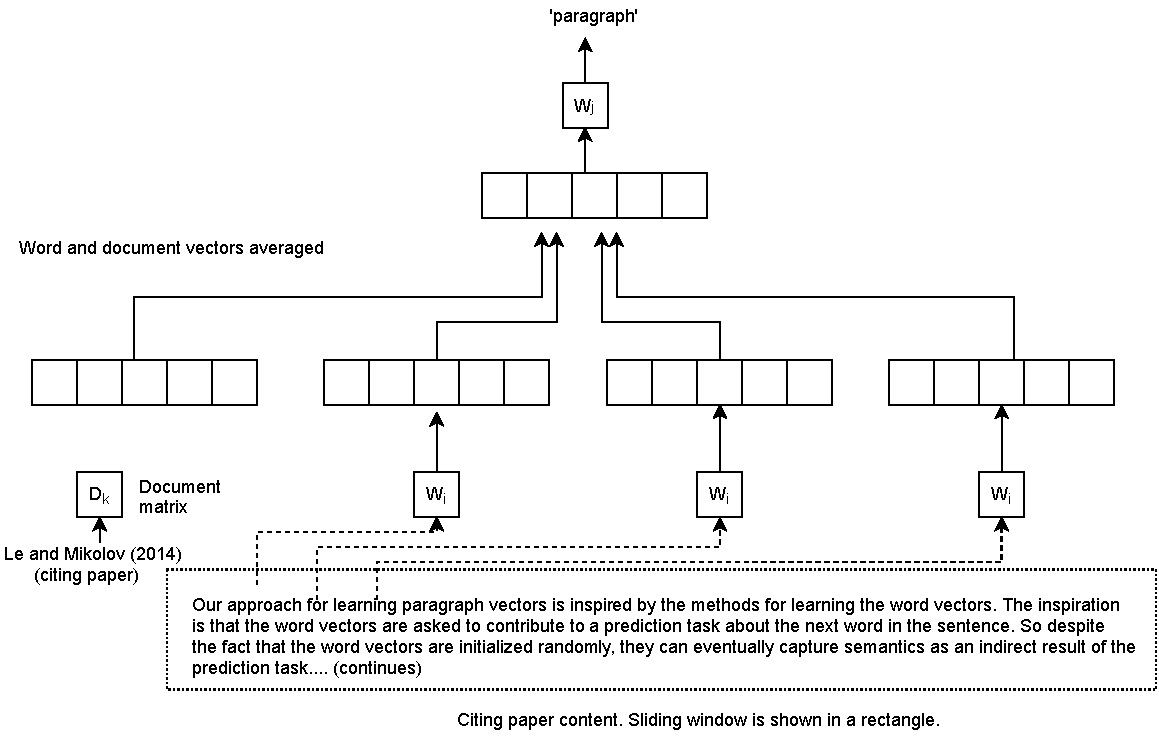
\includegraphics[keepaspectratio, width=13cm]{figures/Approach/pvdm.pdf}
  \caption{Step 1 of Paper2Vec \cite{GangulyP17}: framework for the Doc2vec (pv-dm) model}
  \label{fig:pvdm}
\end{figure}
Before starting Step 2, an intermediate step is carried out in which the set of references for every paper in the training set are obtained. Any references which are not contained within the set are removed. This set of references is obtained during the data preparation phase of Arxiv-MAG, Unpaywall-MAG and ACL-MAG as a by-product. For the MAG data sets, the references are obtained directly from a table containing paper references. These references form a citation graph G = <V,E> with a link appearing between two papers when one cites the other. These edges are assumed to be undirected. So, A citing B is equivalent to B citing A.

\begin{figure}
\centering
 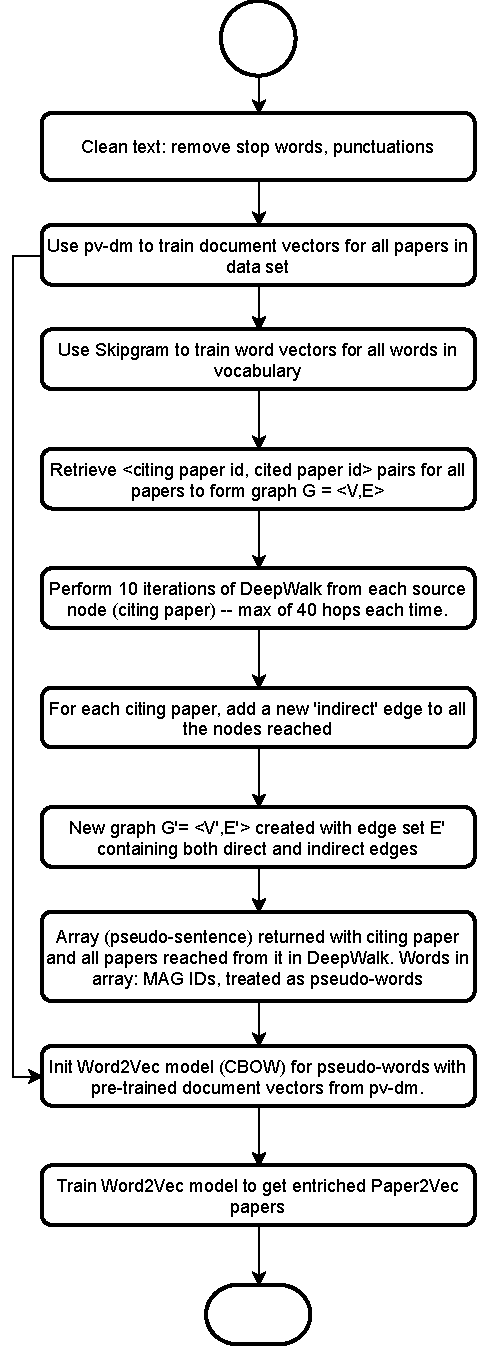
\includegraphics[keepaspectratio, width=8cm]{figures/Approach/paper2vecflowchart.pdf}
  \caption{Flowchart: Paper2Vec~\cite{GangulyP17} training process}
  \label{fig:p2vtrain}
\end{figure}
The document vectors are enriched in Step 2 by creating additional links between the papers through a random walk (based on DeepWalk \cite{PerozziAS14}) step. The graph from the intermediate step contains a number of edges (one edge for each citing-cited paper link)in set E. DeepWalk uses two hyperparamteters for its random walk step: 'number of walks', and 'path length'. 
The 'number of walks' hyperparameter indicates how many times the random walk process should run for a citing paper. The 'path length' hyperparameter indicates how many hops are made in one random walk (DeepWalk) step. Path length is set to 40 and number of walks is set to 10 for all the data sets used in this thesis.

DeepWalk works as follows. The source node (citing paper) of each edge is taken as a starting point and a maximum of 40 hops are made (if an unconnected node is reached, the random walk process ends). This is repeated for 10 iterations. All the nodes reached are returned as an array, and an edge is created between the citing paper (source node) and the nodes reached from it in the 10 DeepWalk iterations. \\
So the new graph at this point is G' = <V, E'> with E' containing the edges in E and all the new edges created during the DeepWalk process. For each citing paper, DeepWalk returns an array containing all the papers reachable from it. These arrays are treated as pseudo-sentences and passed to a Word2Vec CBOW model with negative sampling. The vectors for each pseudo-word (MAG paper IDs) are initialised using the corresponding Doc2vec (pv-dm) vectors produced in Step 1.\\
The idea is that we start from each node in G', and predict each node from its neighbours. The model is trained for a few epochs (5) after the initialising the vectors from those produced in Step 1.
The log probability of the following function is maximised: 
\begin{equation}
    P(v_j|{v_i}) = \frac{exp(v_j^Tv_i)}{\sum_{t=1}^{C_2}{exp(v_t^Tv_i)}}
\end{equation}
where $C_2$ is the set of nodes reached from the source node $v_i$ in 40 or fewer hops.\\
At this stage, we have a set of document vectors of higher quality than the vectors produced after Step 1. But as we will see in Chapter 6, the Paper2Vec method does not work as well as the other methods that will be discussed shortly.\\
Most of the hyperparameters for Step 1 and Step 2 have been left to the values suggested by the original authors. Changes made to optimise them did not have much of an effect. These values are shown in Table~\ref{tab:paper2vechyperparams}. The vector size is varied based on the size of the data set. These vector sizes are given in Table~\ref{tab:paper2vecvectorsize}.

\begin{table}
\centering
\caption{Common Hyperparameters across data sets Paper2Vec}
\label{tab:paper2vechyperparams}
\begin{footnotesize}
\begin{tabular}{ll@{}c}
\toprule
Hyperparameter & Value \\
\midrule
Learning rate for Doc2vec & reduced iteratively from 0.025 to 0.005 \\
Context window size & 10 \\
Mininum Freq. for word to be in vocabulary & 5 (4 for MAG50) \\
Subsampling rate &  0.0001 \\
Number of Random walks & 10 \\
Number of hops in random walk (path length) & 40 \\
Window for Paper2Vec (Word2vec with MAG paper ids) & 5\\
\bottomrule
\end{tabular}
\end{footnotesize}
\end{table}
\begin{table}
\centering
\caption{Vector sizes for Paper2Vec}
\label{tab:paper2vecvectorsize}
\begin{footnotesize}
\begin{tabular}{ll@{}c}
\toprule
Data set & Vector size \\ % Type of cit. rec.
\midrule
ACL-MAG. & 300 \\
Arxiv-MAG. & 500  \\
MAG. & 500 \\
MAG50. & 300 \\
Unpaywall-MAG & 500 \\
\bottomrule
\end{tabular}
\end{footnotesize}
\end{table}
\subsection{Testing process}
Let the set of contexts in the test set be $C_3$. The contexts are first cleaned (the words are converted to lower-case, stop words, special characters and extra white spaces are removed, contractions are expanded). Only contexts whose ground truth contains a paper is in the training set are retained. 
The actual method of prediction is as follows. The IN word vectors (described in Chapter 3) of all the words in the context (after cleaning) are obtained from the vocabulary of the model produced in Step 1 of training. These IN vectors are summed up (the result is a vector) and normalised by the number of word vectors. 
\begin{equation}
    V = \frac{1}{|W|} \sum\limits_{i}^{|W|} w_i
\end{equation}
where W contains the word vectors for the words from the citation context, and the sum is an element-wise sum.
The probabilities of recommending every paper in the training set is obtained by taking a dot product of the aforementioned vector of sums with the document vector matrix from Step 2 of training. This, after normalisation, returns a vector of |n| probabilities. This vector is sorted in descending order of probabilities and the top n papers are recommended.
\begin{equation}
    prob = exp(V . D^T) 
\end{equation}
where prob, the probabilities of all the papers being recommended, is thereafter normalised by the sum of probabilities. D is the document vector matrix.
The prediction process is shown as a flowchart in Figure~\ref{fig:p2vtest}.
\begin{figure}
\centering
 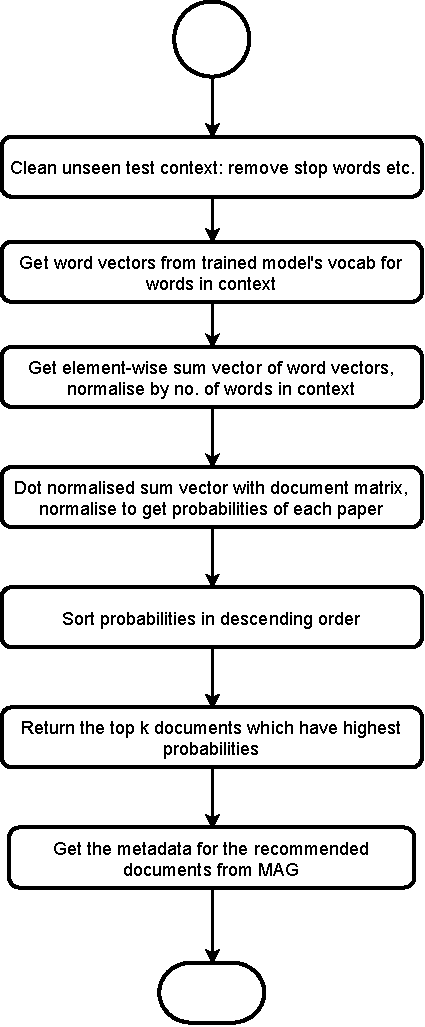
\includegraphics[width=7cm]{figures/Approach/Paper2vectest.pdf}
  \caption{Flowchart: Paper2Vec prediction}
  \label{fig:p2vtest}
\end{figure}
\section{Dual embeddings for hyper-documents: Hyperdoc2vec}
\subsection{Training process}
The Hyperdoc2Vec approach explained in Han et al.~\cite{ShiSZZH18} is a citation recommendation approach which produces two sets of vectors for each paper: IN vectors and OUT vectors (called syn0 and syn1/syn1neg respectively in the popular gensim package). The idea of using dual word embeddings originally comes from \cite{NalisnickMCC16}, in which it is claimed that two vectors work better than one for a variety of tasks. 

Figure~\ref{fig:hd2v} shows the framework for training Hyperdoc2Vec.
Each paper is called a hyper-document in \cite{ShiSZZH18}, as it contains content words as well as annotations (citation markers) which link to other papers. As one of the purposes of the original Hyperdoc2Vec paper is to recommend papers which have not been cited before, it would seem to be a good option to use in the final hybrid algorithm. 
\begin{figure}
\centering
 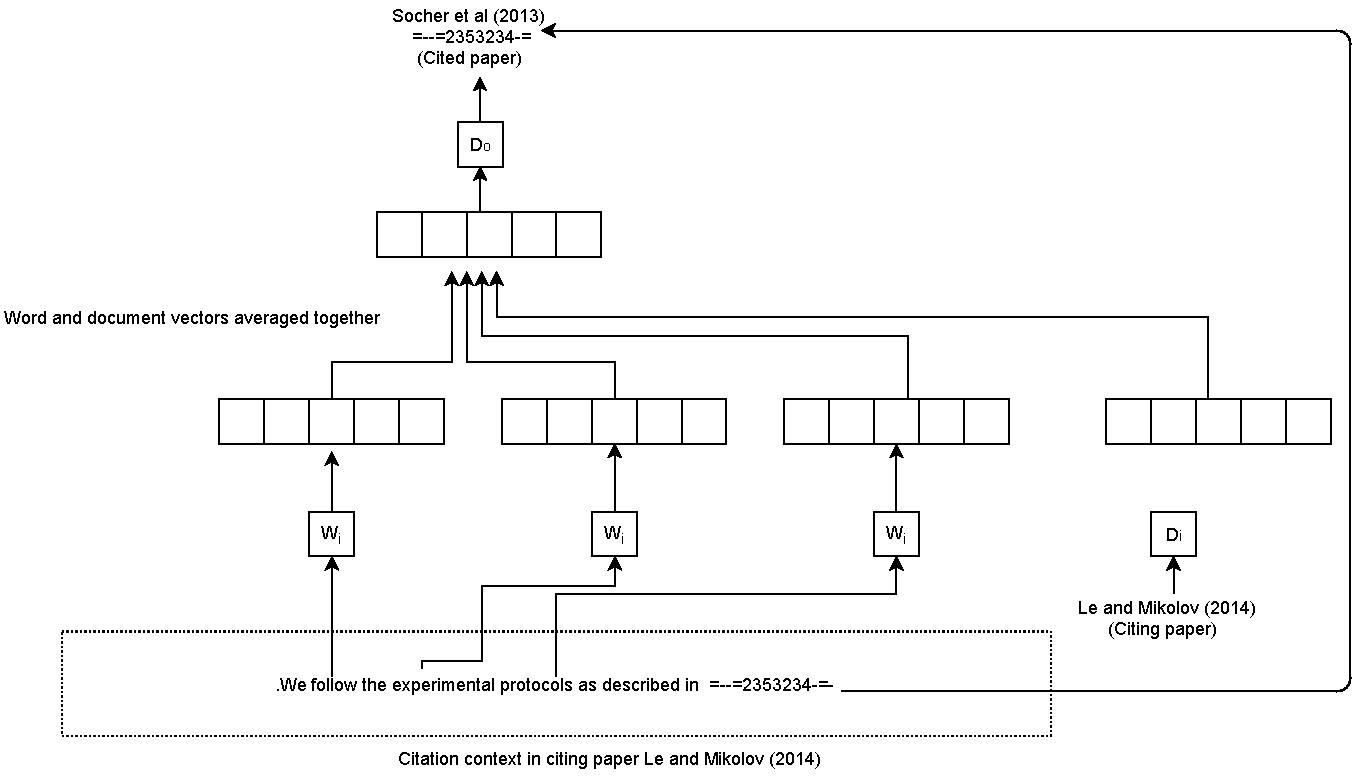
\includegraphics[keepaspectratio, width=13cm]{figures/Approach/hd2v.pdf}
  \caption{Framework for the Hyperdoc2Vec~\cite{ShiSZZH18} model}
  \label{fig:hd2v}
\end{figure}

Before we describe the theory behind the training process, it might be worth mentioning the preprocessing done before training. Like in Paper2Vec, we make words lower-case, remove stop words, expand contractions and remove extra white spaces from the files created in Chapter 4. Appendix~\ref{chap:preprocessing} shows the stop words removed, and explains the preprocessing step in detail.

The entire training process based on~\cite{ShiSZZH18} is shown in the form of a flowchart in Figure~\ref{fig:hd2vtraining}.
In the Hyperdoc2vec approach, for a paper 'P', the IN document vector ($d^I$) represents P playing the role of a source (citing) document. The OUT document vector ($d^O$) represents P playing the role of a target (cited) document. Essentially, this means that the algorithm is both content-aware and context-aware. Both the content of P and the contexts of the papers which cite P play a role in P's embeddings. 

This can be contrasted with the regular Doc2Vec (pv-dm) algorithm described in Section 5.1.1, in which only the IN vectors are generally used. pv-dm is not context-aware, the OUT vectors play no role. 
\begin{figure}
\centering
 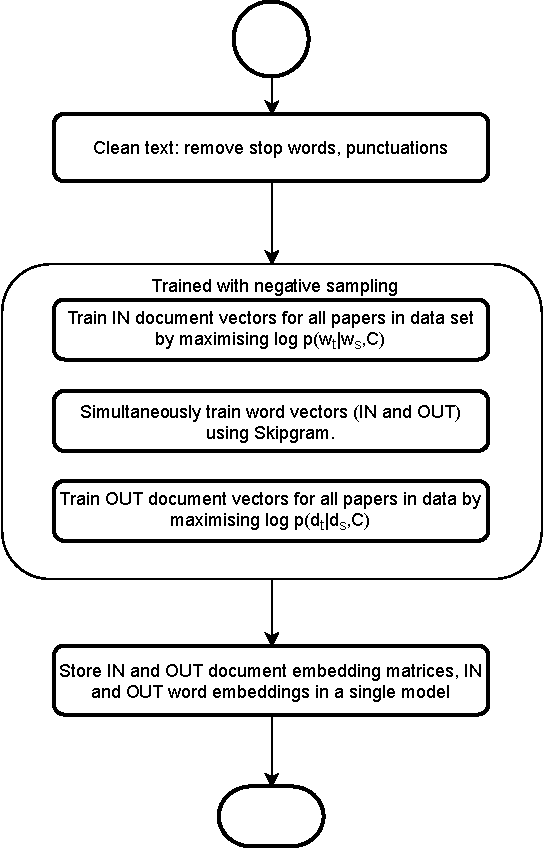
\includegraphics[keepaspectratio, width=8cm]{figures/Approach/hd2vtrainflowchart.pdf}
  \caption{Flowchart: Hyperdoc2vec~\cite{ShiSZZH18} training process}
  \label{fig:hd2vtraining}
\end{figure}
pv-dm maximises $\sum\limits_{w_i, w_j \in c_1}^{|C_1|} log P(w_j|{w_i, d_k})$, the probability of a word given the neighbouring words and the document vector. 

Hyperdoc2vec maximises 2 separate probabilities. Consider the set of all contexts $C={(d_s, C, d_t)}$. The following log probability which models the contexts' impact on the embeddings is the first probability that is maximised: 
\begin{equation}
    \underset{D^I, D^O, W^I}{\max}\; \frac{1}{|C|} \; \sum\limits_{(d_s,C,d_t) \in C}\: log P(d_t|d_s, C)
\end{equation} 
where $D_I$, $D_O$ and $W_I$ are the set of all IN and OUT document vectors, and word vectors respectively. 
\begin{table}
\centering
\caption{Common Hyperparameters across data sets Hyperdoc2Vec}
\label{tab:hd2vhyperparams}
\begin{footnotesize}
\begin{tabular}{ll@{}c}
\toprule
Hyperparameter & Value \\
\midrule
Learning rate &  0.025 \\
Number of training iterations & 100 \\
Half-context window size & 20 \\
Subsampling rate (negative sampling) &  0.001 \\
Vector size & 300 (but 100 for ACL-MAG) \\
\bottomrule
\end{tabular}
\end{footnotesize}
\end{table}
The probability that a cited document $d_t$ is cited in a context C of a citing paper $d_s$ is modelled by averaging the IN word vectors of the words in the context.
\begin{equation}
    x = \frac{1}{1+|C|} (d_S^I + \sum\limits_{w\in C} w^I)
\end{equation}
Finally, this average of vectors is combined with the OUT document vectors to implement a multi-class softmax classifier (as in Section 5.1).
\begin{equation}
    P(d_t|d_s, C) = \frac{exp(x^T d+t^O)}{\sum\limits_{d\in D} exp(x^Td^O)}
\end{equation}
The contents' impact on the papers' embeddings is also modelled. This is done by predicting the OUT word vector of each word from the neighbouring word and the document vector, as in pv-dm. The equation for a source document $d_s$ is: 
\begin{equation}
    P(w_j|{w_i, d_s}) = \frac{exp(w_j^Tw_i + w_j^td_s)}{\sum_{t=1}^{C_1}{exp(w_t^Tw_i + w_t^Td_s)}}
\end{equation}
Here, $w_j$ is the 'current' word vector, and the word vectors of the other words in the same context are represented by $w_i$.
The following equation is maximised: 
\begin{equation}
    \sum\limits_{w_i, w_j \in c_1}^{|C_1|} log P(w_j|{w_i, d_k})
\end{equation}
\begin{figure}
\centering
 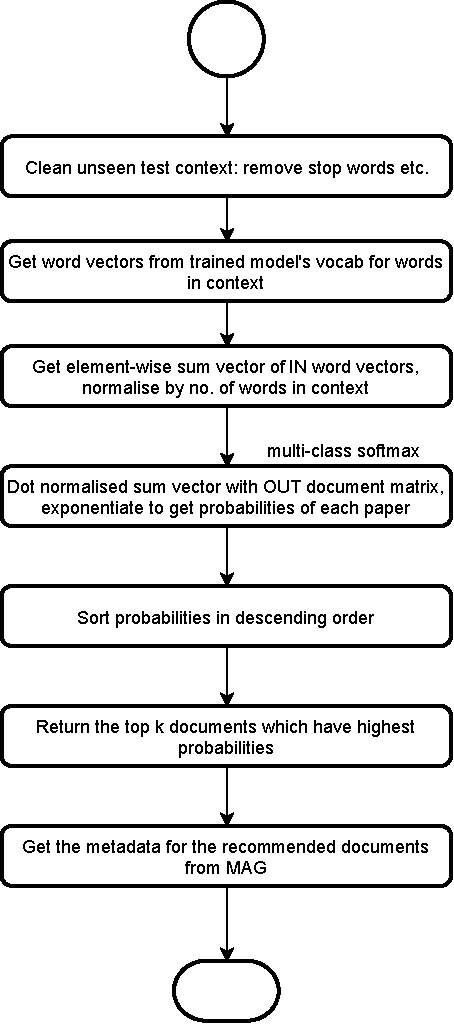
\includegraphics[width=7cm]{figures/Approach/hd2vOUT.pdf}
  \caption{Flowchart: Prediction using Hyperdoc2vec OUT document vectors and IN word vectors of context (hd2vOUT)}
  \label{fig:hd2vOUT}
\end{figure}
The main hyperparameters used are the vector size and the size of the context window. The hyperparameter for calculating the size of the context window is the 'half-context window'. The half-context window used for all the data sets is 20 in this thesis. This means that the citation context is made up of 40 words while training the algorithm. Experiments showed that this worked well as the average citation context length seemed to be around 40. The vector sizes are kept constant for all the data sets except the small ACL-MAG data set. The hyperparameters used are shown in Table~\ref{tab:hd2vhyperparams}.\\
In this thesis, we divide the Hyperdoc2Vec algorithm into two for the testing and evaluation phases based on which vectors are used. When only the OUT document vectors are used, we call the algorithm hd2vOUT. When both IN and OUT document vectors are used, we call the algorithm hd2vINOUT.

\subsection{Testing process}
There are 4 possible combinations of document and word vectors which we can choose from. The first option is to use a multi-class softmax classifier after taking a dot product of the OUT document matrix (made up of OUT document vectors) and the average of the IN vectors of the context words. This is shown in equation (8). The multi-class softmax classifier returns a probability for each paper in the training corpus. These probabilities are sorted and the top n recommendations are returned. This version of the algorithm is called hd2vOUT and the complete process is sketched out as a flowchart in Figure~\ref{fig:hd2vOUT}.

The other three combinations (OUT document vectors and OUT word vectors, IN document vectors and IN word vectors, IN document vectors and OUT word vectors) do not work as well as the first option. 

Another thing we can do is to use the embeddings based on both the contents and the contexts and feed this to another multi-class softmax classifier. This is done by taking the dot product the averaged IN word vectors of the context with the OUT document matrix, taking the dot product of the averaged OUT word vectors of the context and the IN document matrix, and adding the two vectors together. A final exponentiation completes the process.
As before, this multi-class softmax classifier also returns a probability for each paper in the training corpus. These probabilities are sorted and the top n recommendations are returned. This version of the algorithm is called hd2vINOUT and the process is shown in Figure~\ref{fig:hd2vINOUT}.
\begin{figure}
\centering
 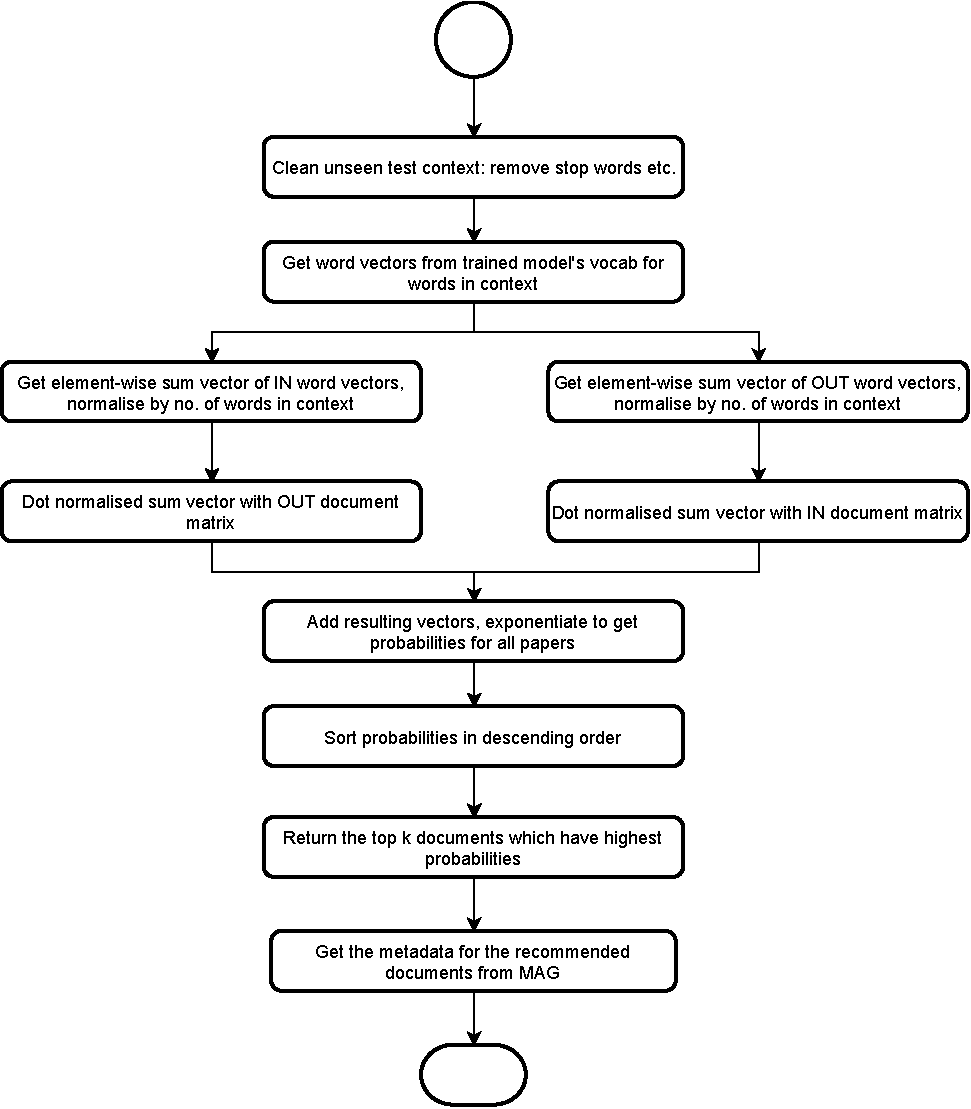
\includegraphics[width=15cm,height=17cm]{figures/Approach/hd2vINOUT.pdf}
  \caption{Flowchart: Prediction using Hyperdoc2vec OUT document vectors and IN word vectors of context, IN document vectors and OUT word vectors (hd2vINOUT)}
  \label{fig:hd2vINOUT}
\end{figure}

As we will see in the next chapter (chapter 6), using the OUT document vectors with the IN word vectors is the method that works best of all. Using both the IN and OUT document vectors doesn't work as well in practice.
\section{Topic Modelling and Information Retrieval algorithms}
\subsection{Similar topic models using LDA}
The idea behind using the Latent Dirichlet Allocation (LDA) \cite{BleiNJ03} for citation recommendation is to recommend papers whose content maps to a similar set of topics as those of the test citation context. The flowchart for the LDA training process is given in Figure~\ref{fig:ldatrainingflowchart}.
\begin{figure}[h]
\centering
     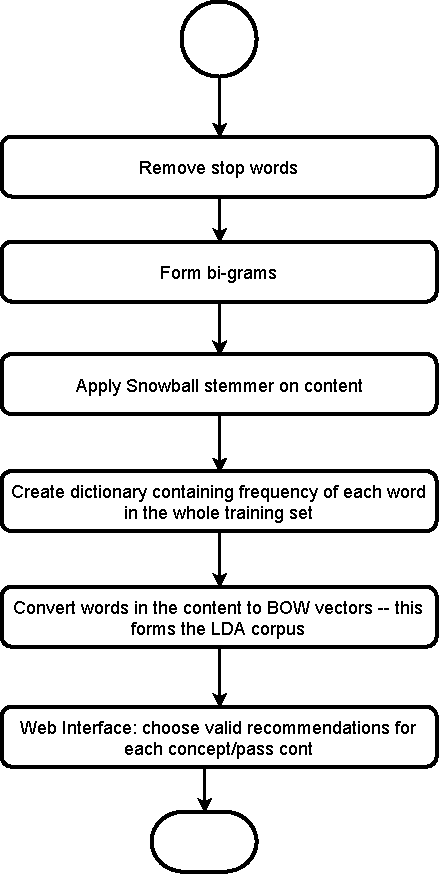
\includegraphics[width=6cm]{figures/Approach/LDAtrainingflowchart.pdf}
  \caption{Flowchart: LDA Training process}
  \label{fig:ldatrainingflowchart}
\end{figure}
\begin{figure}
 \centering
 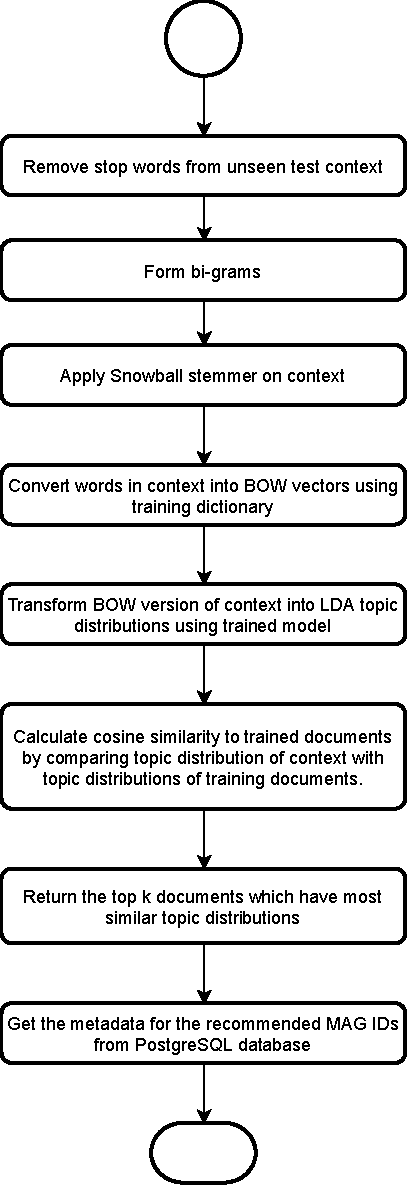
\includegraphics[width=6cm]{figures/Approach/LDAtestingFlowchart.pdf}
  \caption{Flowchart: LDA Prediction}
  \label{fig:ldapredictflowchart}
\end{figure}
The Gensim package is used for getting the topic models. It was found during testing that the MALLET implementation of LDA \footnote{http://mallet.cs.umass.edu/} produced higher-quality topic models than the normal Gensim version of LDA. The difference between MALLET and the normal Gensim LDA is that MALLET uses Gibbs sampling while the normal Gensim LDA uses a Variational Bayes sampling method. While Gibbs sampling is more precise, MALLET takes an inordinate and impractical amount of time for prediction. Therefore, it was decided to use only the normal LDA during evaluation. However, the LDA Mallet is evaluated in Chapter 6 for the smallest ACL-MAG data set, and it performs slightly better than the normal LDA (but much worse than most of the other non-LDA algorithms).\\
The first step to use LDA for citation recommendation is the preprocessing step. This is much more complex than the preprocessing done for the embedding algorithms. Stop words are removed first, and then bi-grams are created. This is then followed by a stemming process using the Snowball stemmer. 
Once this is done, the dictionary and the corpus for LDA can be built. The dictionary maps words to their frequencies over the whole training set. The corpus contains bag-of-words representations of all the documents. The topic model is created from the dictionary and corpus. The number of topics is a hyperparameter which has to be chosen. In this thesis, experiments were done with between 100 and 500 topics and the perplexity was calculated. The number of topics used finally was 300 for all the large data sets and 200 for the small ACL-MAG data set.

The same preprocessing is performed while doing the prediction and evaluation on a citation context, and the words in the context are mapped to topics. After converting this context into a bag of words, we compare the topics of the context with the topics of all the papers in the training set using cosine similarity. The similarities are sorted in descending order, and the top n similar papers are recommended.
The flowchart for the LDA testing process is given in Figure~\ref{fig:ldapredictflowchart}.
\subsection{BM25}
The famous Okapi BM25 algorithm is a bag-of-words algorithm used in citation recommendation approaches, sometimes as a pre-filter and sometimes as a simple baseline. BM25 ranks returned documents based on the query terms appearing in each document. However, the specific position of the query terms makes no difference to the ranking function. For example, if the query terms are 'information', 'retrieval' and 'technique', it will assign the same score to two different documents which have the three words the same number of times, but in different order. 

\begin{figure}
\centering
 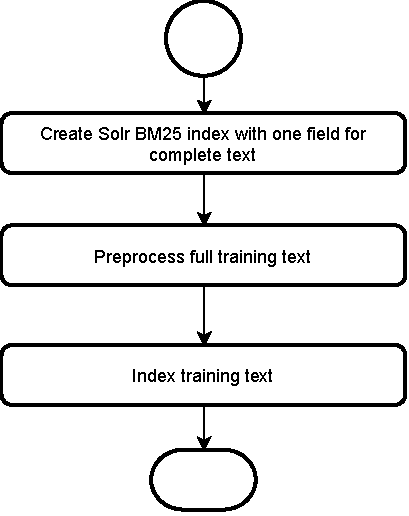
\includegraphics[width=6cm]{figures/Approach/bm25trainingflowchart.pdf}
  \caption{Flowchart: Solr BM25 Training process}
  \label{fig:bm25trainingflowchart}
\end{figure}
To implement BM25, the open-source indexing engine Apache Solr (which runs on Apache Lucene) is used. After preprocessing, the entire content of the document, whether it is from MAG or the other data sets, is indexed in Solr in a single field. 
The training process for BM25 is given in Figure~\ref{fig:bm25trainingflowchart}.
\begin{figure}[h]
 \centering
 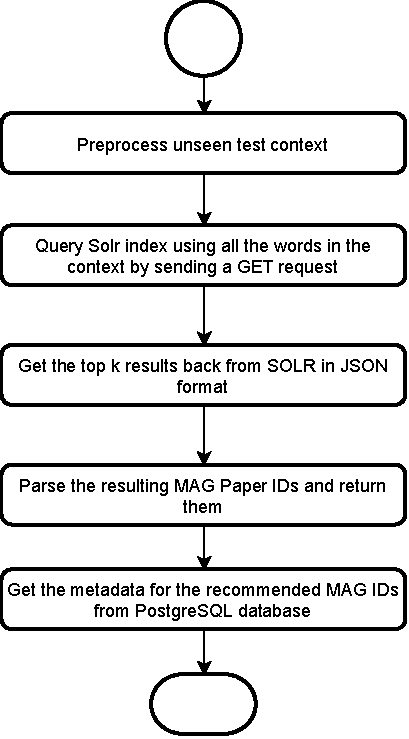
\includegraphics[width=6cm]{figures/Approach/bm25testflowchart.pdf}
  \caption{Flowchart: BM25 Prediction}
  \label{fig:bm25predictflowchart}
\end{figure}
While testing, the queries are constructed as a simple query consisting of all the terms in the preprocessed citation context. A GET request is sent to Solr with the words as parameters, and the top n results are returned. The similarity used while comparing the BM25 vectors is, like in the case of LDA, cosine similarity. 
The flowchart for the BM25 prediction process is given in Figure~\ref{fig:bm25predictflowchart}.\\
The MAG-Cited data set described in Section 4.2.6 is also indexed in the same way as Figure~\ref{fig:bm25trainingflowchart} so that it can be used in the improved hybrid algorithm in Section 5.5 and the case study in Section 6.2.4. The testing process for the MAG-Cited data set is also exactly the same as described in Figure~\ref{fig:bm25predictflowchart}.

\section{Semi-genetic Hybrid recommeder for Citation recommendation}
Recommendations from different recommender systems can be combined in many ways. It can be as simple as giving scores to each recommender system's recommendations based on ranks, and adding the scores for items which have been recommended by both recommender systems. However, there are a number of questions which can be raised in this case. Is an item that is ranked 50 and 80 by two recommender systems a better candidate than another item which has been ranked 5 and 240? How should we score items which have been ranked highly (say, 2) by one recommender system, but which haven't been returned at all by the second recommender system. These are questions with no obvious answers.

An interesting option would be to use a weighted hybrid algorithm which combines recommendations stochastically.  Mueller~\cite{Mueller17} describes one such algorithm which can be used to construct a 'semi-genetic' hybrid recommender. The algorithm is called 'semi-genetic' because it uses only some of the steps of the genetic algorithm explained in Chapter 3. The cross-over and mutation steps of genetic algorithms are skipped. In addition, the semi-genetic algorithm has only one iteration, unlike most genetic algorithms. 
In this thesis, we implement this algorithm to build a semi-genetric hybrid citation recommendation system. A flowchart of our hybrid citation recommendation system is shown in Figure~\ref{fig:hybridflowchart}.

The recommendations from the best individual algorithms described previously are fed into this semi-genetic hybridisation algorithm. Experiments conducted across data sets (the evaluations results are described in Chapter 6) indicate that some of the algorithms do a lot better than others. Using all the algorithms as part of the hybrid recommender did not increase its recall. For this reason, our hybridisation algorithm combines recommendations from only two individual recommenders -- the BM25 recommender, and the Hyperdoc2vec recommeder with OUT document vectors (hd2vOUT). Using only the OUT vectors (along with the IN word vectors of the words in the context) works almost twice as well as using both the IN and OUT document vectors, as shown in Chapter 6. 

The steps of the semi-genetic hybridisation algorithm for combining BM25 and hd2vOUT recommendations are given below. The process runs for only one iteration, unlike most genetic algorithms.

\textbf{Step 1.} Initialise population: select a set of items from all possible 'chromosomes', i.e. from the recommendation lists of both component algorithms. In this step, we get the top 500 recommendations from BM25 and the top 500 recommendations from hd2vOUT, and concatenate them.

\textbf{Step 2.} Evaluate fitness scores: The reciprocal rank is assigned as the fitness score for the recommendations from each of the algorithms. Using the reciprocal rank is a fair proxy for the fitness score -- if an algorithm ranks a paper highly, it indicates that it gives the paper a high score. For example, if paper A has been ranked 1 by BM25, its fitness score for BM25 is 1/1. If the same paper has been ranked 200 by hd2vOUT, its fitness score for hd2vOUT is 1/200. Let's say Paper B has been ranked 10 by BM25. Then its fitness score for BM25 is 1/10. If Paper B hasn't been returned by hd2vOUT, there is no fitness score associated with it for hd2vOUT. Note that the two component algorithms have been given equal weights in this step.

At this stage, we have an array of 1000 recommendations, 500 from hd2vOUT and 500 from BM25. Each of the recommendations is associated with a fitness score (reciprocal rank). If a paper has been recommended by both algorithms, it will have two scores associated with it.

\textbf{Step 3.} Convert the scores into probabilities. This is done by dividing each score by the sum of all the scores.
\begin{figure}
 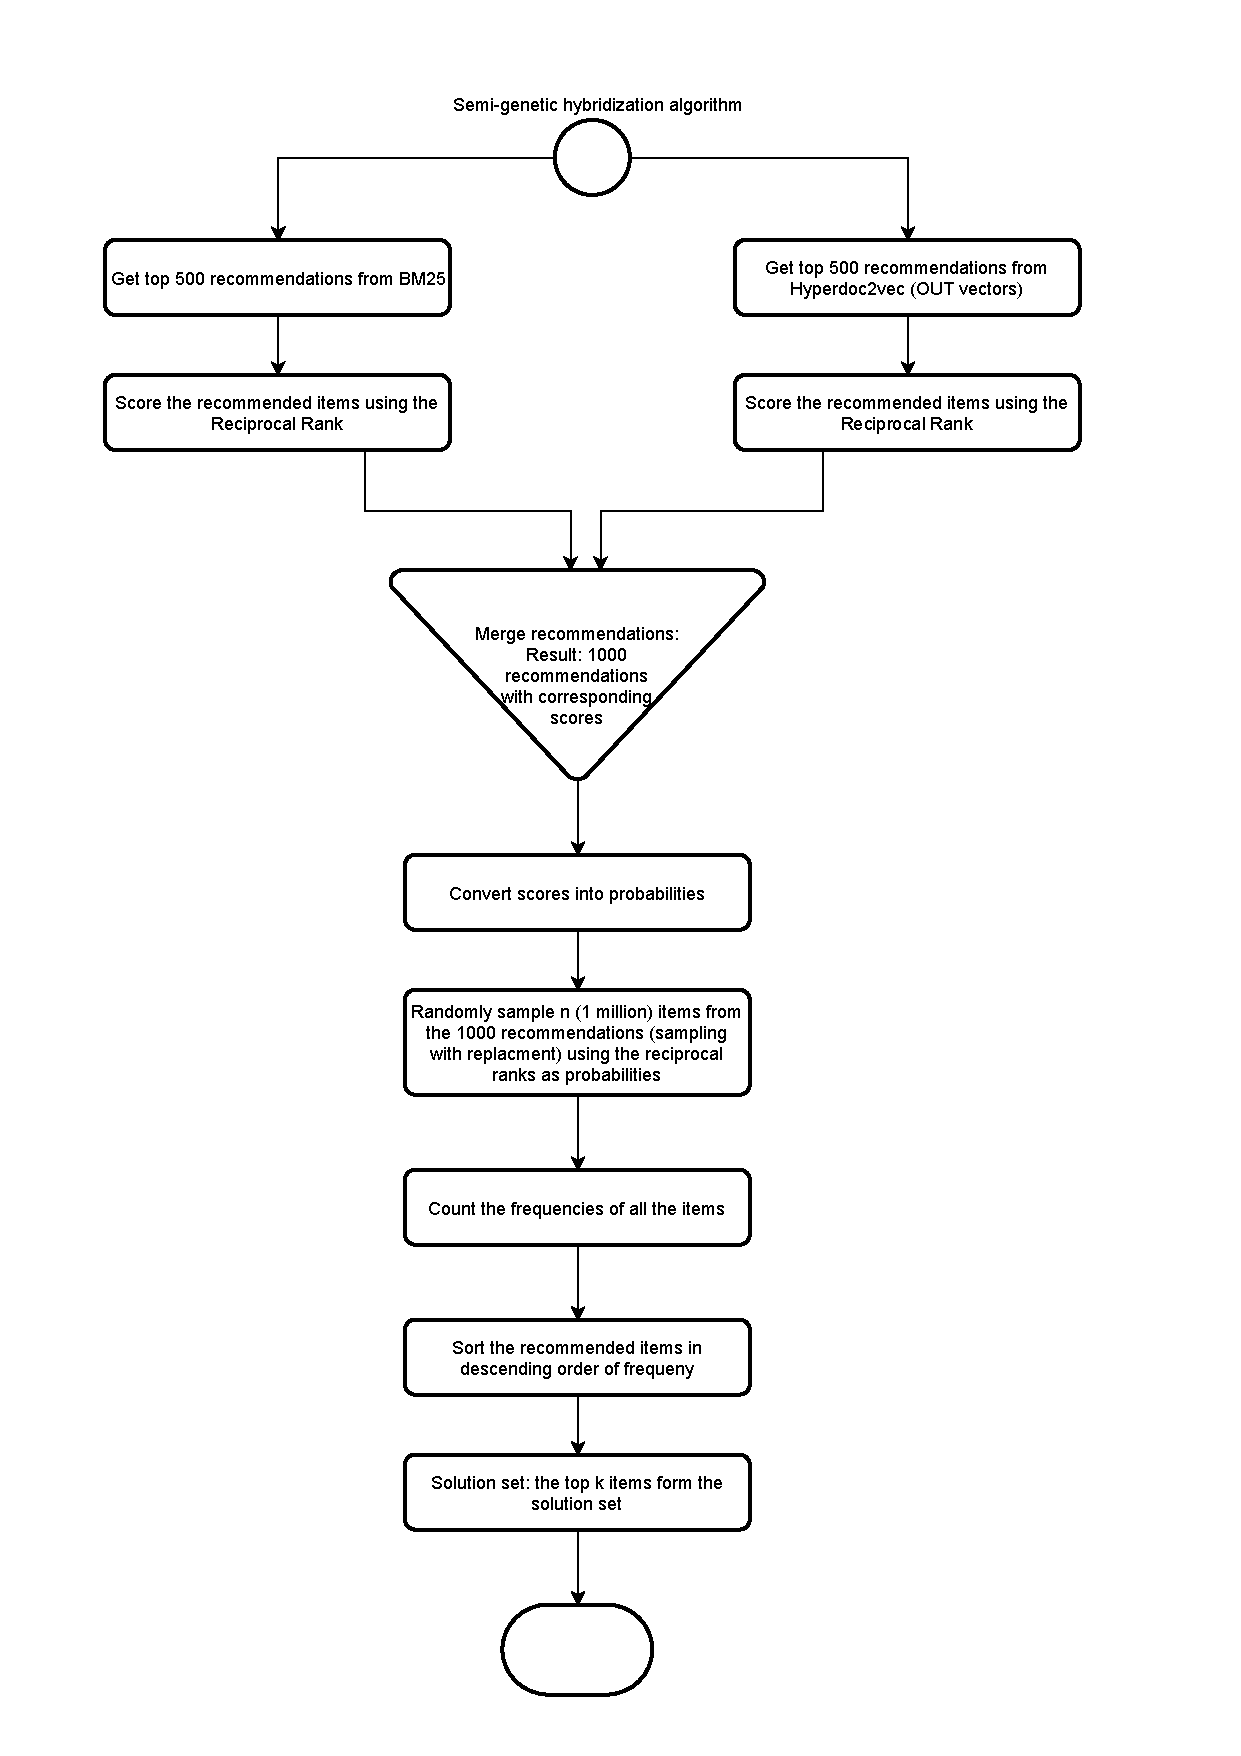
\includegraphics[keepaspectratio, width=14cm]{figures/Approach/Hybridflowchart.pdf}
  \caption{Flowchart: semi-genetic hybridisation algorithm for citation recommendation}
  \label{fig:hybridflowchart}
\end{figure}

\textbf{Step 4.} Selection: we randomly draw n (n = 1 million) samples with replacement from the array of 1000 recommendations. The idea is that papers which have higher ranks in either of the lists will have a higher probability of being drawn in the random sample. Papers which have been recommended by both the component recommenders have two distinct probabilities of being drawn. A paper which has been ranked highly by both algorithms (say 1 and 3) will have a very high probability of being drawn in the random sample.

As the random sample is made with replacement, the best recommendations from both the algorithms combined will be recommended the most number of times. This is a stochastic process, and we expect the random draws to depend on two factors: (i) its probability of being drawn in either algorithm -- the higher the better, (ii) the presence of a paper in both recommendation lists -- however, the individual ranks in each of the lists matter immensely. So, a paper which has been ranked 400 and 500 by the two algorithms may get picked a lot less than a paper which is not present in one algorithm's recommendation list, but has been ranked 2 by the other algorithm.

\textbf{Step 5.} Count the number of times each of the papers is drawn. 

\textbf{Step 6.} Sort the recommendations in descending order of frequencies. 

\textbf{Step 7.} Solution set: at this stage, the sorted array of recommendations will have at most 1000 papers, but usually less than 1000 papers (as the two component algorithms will usually recommend at least some common papers). To get the final solution set, we return the top k recommendation from the sorted array of recommendations.
\section{Hybrid23: Improved Hybrid algorithm based on 2 MAG data sets and 3 components}
While the hybrid algorithm explained in Section 5.4 works better than its individual components, its performance can be improved further by using two data sets. 

The data sets we use for this algorithm are the regular MAG data set described in Section 4.2.2 and the MAG-Cited data set described in Section 4.2.6. The MAG-Cited data set, like the normal MAG data set, contains pseudo full-text for the content of each paper. However, the citation contexts in a paper's pseudo full-text are from papers which cite it. 

The BM25 algorithm performs much better in an offline evaluation on the MAG-Cited data set compared to the MAG data set, as we show in a case study in Section 6.2.4. This is due to the fact that citation contexts tend to describe the cited papers better than the citing papers. Therefore, the text-matching based BM25 algorithm works better when the citation contexts from a citing paper are present in a cited paper's content. 
\begin{figure}
 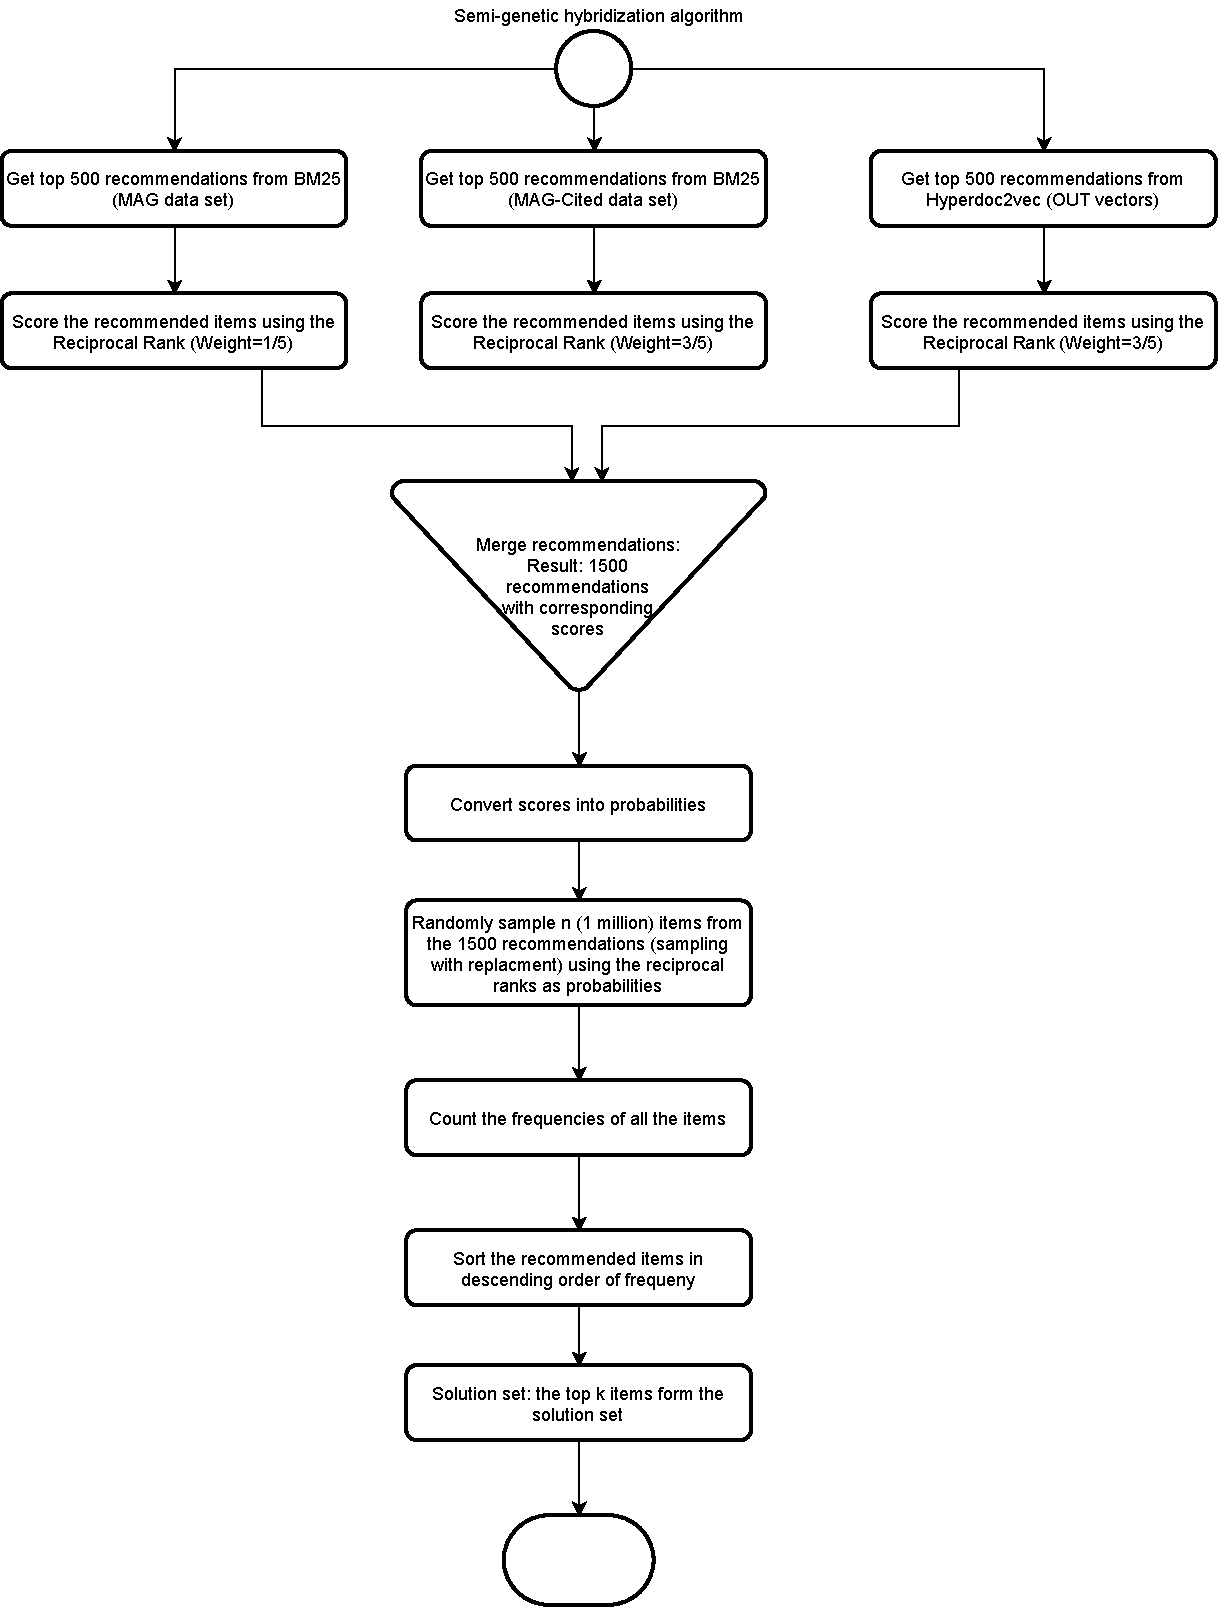
\includegraphics[keepaspectratio, width=14cm]{figures/Approach/hybridv2flowchart.pdf}
  \caption{Flowchart: Hybrid23 -- improved semi-genetic hybridisation algorithm which uses two MAG data sets and three components}
  \label{fig:hybridv2flowchart}
\end{figure}
The improved hybrid recommender system uses the above two data sets and contains three components. It is therefore called \textbf{Hybrid23}. Its three components are:
\begin{enumerate}
    \item hd2vOUT trained on the MAG data set
    \item BM25 trained on the MAG data set
    \item BM25 trained on the MAG-Cited data set
\end{enumerate}
A flowchart for the Hybrid23 is shown in Figure~\ref{fig:hybridv2flowchart}.
The algorithm is almost the same as the one in Section 5.4, but there are changes in Steps 1 and 2 due to the fact that there are three components. The steps are explained below.\\
\textbf{Step 1.} Initialise population: select a set of items from all possible 'chromosomes', i.e. from the recommendation lists of the \textit{three} component algorithms. In this step, we get the top 500 recommendations from BM25 (MAG), hd2vOUT (MAG), BM25 (MAG-Cited) and concatenate them. At the end of this step, we have a list of 1500 recommendations.\\
\textbf{Step 2.} Evaluate fitness scores: The hybrid algorithm in Section 5.4 gave equal weights to the two component algorithms. But now, we have three component algorithms in which one (BM25 for MAG-Cited) works much better than the others. So while the reciprocal rank is still assigned as the fitness score for the recommendations from each of the algorithms, it is weighted differently. The reciprocal ranks for the recommendations from the BM25 algorithm for MAG-Cited are multiplied by a weight of 3/5 (60\%), while the reciprocal ranks of the recommendations from the other two algorithms (BM25 for MAG and hd2vOUT) are multiplied by a weight of 1/5 (20\%) each. 
E.g.: the fitness scores of the second-ranked recommendation from the BM25 (MAG-Cited) component is 3/10, while the fitness scores for the second-ranked recommendation from the other two components are 1/10 and 1/10 respectively. ran At the end of the step, we have 1500 recommendations with their respective fitness scores.\\
\textbf{Steps 3-7} are exactly the same as the algorithm described in Section 5.4, except for the fact that we now have 1500 recommendations instead of 1000 recommendations. The probabilities of picking recommendations from the BM25 (MAG-Cited) component are much higher.

\section{HybridCite: Running Citation Recommendation System}
An online citation recommendation system is created in which the user is allowed to enter free text and get citation recommendations. 
After the observations made during the process of doing the online and offline evaluation (including the case study in Section 6.2.4), the improved hybrid algorithm (Hybrid23) described in Section 5.5 was chosen as the algorithm to use under the hood in the running system. Additionally, it was decided that the users would be given a few options, which will be described shortly.

\begin{figure}
    \centering
    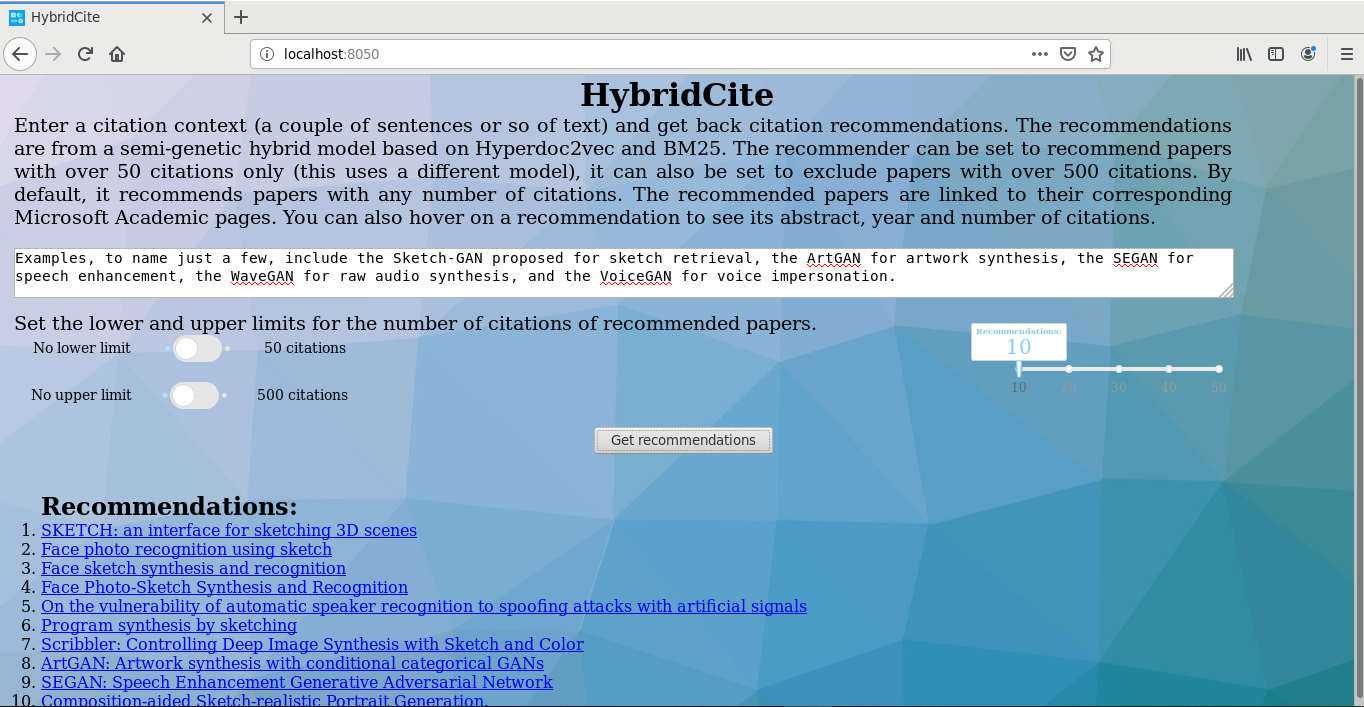
\includegraphics[keepaspectratio, width=13cm]{figures/Approach/recommsystem.PNG}
    \caption{Interface of the citation recommendation system 'HybridCite'}
    \label{fig:hybridcite}
\end{figure}
Two separate models are used in the final recommendation system -- Hybrid23 models trained on the MAG (and MAG-Cited) and MAG50 (and its corresponding reduced version of MAG-Cited) data sets. MAG50 contains only papers which have been cited 50 times or more. The reason for including the MAG50 model is that some users might not want to be recommended papers which haven't been cited much. On the other hand, it is likely that other users might know the popular papers and would want to be recommended more obscure papers. 

The default model used is the one based on the main MAG and MAG-Cited data sets, but users who want to be recommended reasonably well-known papers might want to use the MAG50 model. It is important to note at this stage that the MAG50 model will also miss new papers because they haven't had the time to get 50 citations. 

Another option that is given to the users is to remove very popular papers which have more than 500 citations. It is unlikely that a researcher doing research on word embeddings will want to be recommended the popular Word2Vec paper, or that a person researching uses of SVMs might want to be recommended the original SVM paper. These papers are so popular that most researchers will have heard of them, and the recommendation might not therefore be useful.

Finally, the user can choose to get more than the default 10 recommendations -- he/she can choose to get 20, 30, 40 or 50 recommendations. Each time the number of recommendations is changed, new recommendations are retrieved and the page is dynamically updated. This involves getting fresh recommendations from hd2vOUT and the two BM25 implementations, and combining them again using the hybrid algorithm. It is entirely possible (and probable) that the recommendations in the new list retrieved from the hybrid algorithm might be in a different order to the previous list. The hd2vOUT and BM25 algorithms might return recommendations in slightly different order, and the stochastic hybrid algorithm may select different papers in its result set. So if the user gets 10 recommendations, and later changes the number of recommendations to 20, the papers at the top of the list might be different from the ones at the top of the list when 10 recommendations were retrieved.

The interface of the recommendation system is shown in Figure~\ref{fig:hybridcite}. The recommended papers returned are linked to their corresponding pages on Microsoft Academic. The abstract, published year and the citation count are visible as a tooltip when the user hovers on the link to the recommended paper. These citation counts are as per the values currently in the underlying database and might not match the citation counts on the latest Microsoft Academic page.